\chapter{Conceitos}
\label{cap:conceitos}

A Internet se popularizou de tal maneira que tornou-se essencial para a nossa sociedade, com o grande crescimento da Internet, cresce também a preocupação com as informações que trafegam nas redes de computadores. De acordo com \citeonline{nunes2012definiccao}, ataques com o objetivo de prejudicar o funcionamento de redes de computadores e sistemas de informação têm  crescido tanto em número quanto em impacto. Especialistas têm estudado cada vez mais os meios para proteger as informações e sistemas contidos nas redes de computadores. A proteção de computadores e todos o seus componentes é chamada de cibersegurança. Porém, de acordo com \citeonline{fischer2014cybersecurity} é difícil encontrar uma definição exata para cibersegurança, ela geralmente se refere a um ou mais dos seguintes itens:
\begin{enumerate}
    \item Um conjunto de atividades e medidas que visam proteger (de ataques, interrupções, ou outras ameaças) computadores, redes de computadores, ou qualquer software ou hardware relacionado;
    \item A proteção resultante mediante ao uso de tais medidas;
    \item Um amplo campo de atuação, focado na pesquisa e implementação das atividades e medidas de proteção citadas no item 1.
\end{enumerate}

Portanto, para o melhor entendimento do conceito de cibersegurança, é necessário saber quais e o que são as vulnerabilidades e ameaças que podem pôr em risco a segurança dos dispositivos de redes. Deste modo, este capítulo apresentará brevemente as definições de vulnerabilidades e ameaças. Além disso, será discutido sobre as ferramentas utilizadas e tecnologias que embasam este trabalho.



%A Internet vem se tornando cada vez mais popular com o passar dos anos e juntamente com ela, vem a preocupação com a informação digital, especialistas na área vem se esforçando cada vez mais para proteger essas informações. A proteção de computadores e todos o seus componentes, incluindo a informação, é chamada de cibersegurança. Porém é difícil encontrar uma definição exata para cibersegurança, portanto, de acordo com \citeonline{fischer2014cybersecurity} ela geralmente se refere a um ou mais dos seguintes itens:
%\begin{enumerate}
%   \item Um conjunto de atividades e medidas que visam proteger (de ataques, interrupções, ou outras ameaças) computadores, redes de computadores, ou qualquer software ou hardware relacionado.
 %   \item A proteção resultante mediante ao uso de tais medidas.
 %   \item Um amplo campo de atuação, focado na pesquisa e implementação das atividades e medidas de proteção citadas no item 1. 
%\end{enumerate}


%Portanto, a proteção contra vulnerabilidades e ameaçs de quaisquer dispositivos, tanto  conectados à Internet quanto em quaisquer outras redes de computadores é um ponto basico da cybersegurança. Porém, para realizar uma proteção eficiente dos dispositivos de redes é necessario entender um pouco mais sobre tais vulnerabilidades e ameaças. Neste capitulo, será discutido brevemente os conceitos de vulnerabilidades e ameças, além disso, também sera comentando sobre as ferramentas utilizadas para a realização do objetivo proposto neste trabalho.  
%---------------------------------------------------%

\section{Ameaças}
\label{ameaças}
Para \citeonline{bishop2005introduction} ameaça é tudo o que pode potencialmente violar a segurança de sistemas, ou seja, tudo aquilo que de maneira intencional, ou não, pode disparar vulnerabilidades e causar impactos nos sistemas afetados.
Segundo \citeonline{nla.cat-vn3850333} as ameaças podem ser classificadas como:
\begin{itemize}
    \item Ameaças Naturais: Causados por fenômenos naturais, ocorrem sem a intervenção humana, como por exemplo, enchentes, terremotos, tempestades, incêndios naturais, entre outras;
    \item Ameaças Humanas: Causados por seres humanos, podemos dividir estas ameaças em dois tipos, voluntárias e involuntárias. Ameaças voluntárias ocorrem quando existe a intenção de executar uma ação maliciosa, como por exemplo, \textit{hackers} que procuram roubar informações. Ameaças involuntárias ocorrem quando não há nenhuma intenção maliciosa envolvida; %dar exemplos de voluntário e involuntário
    \item Ameaças Ambientais: Riscos que ocorrem devido ao ambiente em que os sistemas se encontram, como por exemplo, picos de energia, poluição, vazamento de líquidos, entre outros.
\end{itemize}
As ameaças não apresentam riscos caso não existam vulnerabilidades que possam ser disparadas (ameaças naturais, ameaças ambientais ou ameaças humanas involuntárias) ou exploradas (ameaças humanas voluntárias). Por exemplo, a ameaça ambiental de queda de energia não apresenta nenhum risco para um computador que esteja ligado em um \textit{nobreak}. Portanto, para diminuir os riscos que as ameaças representam  deve-se diminuir as vulnerabilidades existentes em redes ou sistemas de computadores. Deste modo é necessário entender o que são vulnerabilidades.



%---------------------------------------------------%
\section{Vulnerabilidades}
\label{vulnerabilidades:ameaças}
De acordo com \citeonline{nla.cat-vn3850333} vulnerabilidades são fraquezas ou falhas de segurança no projeto, implementação, operação ou gerenciamento de sistemas, podem ser acidentalmente desencadeadas ou intencionalmente exploradas, resultando em brechas ou violações na segurança de sistemas. Algumas vulnerabilidades, quando exploradas, permitem que  usuários não autorizados obtenham o controle de sistemas, podendo assim realizar várias ações maliciosas, como por exemplo, realizar novos ataques, além de obter acesso a informações confidenciais que podem gerar grandes prejuízos. \cite{nakamura2007segurancca}.

Este trabalho tem foco nas vulnerabilidades que podem ser exploradas, como por exemplo, programas desatualizados, senhas de autenticação fracas, entre outras. Tais vulnerabilidades podem ser descobertas com a ajuda de algumas ferramentas, chamadas de \textit{scanners}, ferramentas que podem ajudar tanto o atacante quanto o defensor, os atacantes utilizam os \textit{scanners} para localizar e então explorar as vulnerabilidades, enquanto  os defensores utilizam  os \textit{scanners} para localizar e corrigir as vulnerabilidades encontradas \cite{fischer2014cybersecurity}.

%---------------------------------------------------%
\section{Ferramentas de análise de vulnerabilidades}
\label{cap:conceitos:sec:Ferramentas}
Segundo \citeonline{weidman2014penetration}, a maioria das empresas com orçamentos consideráveis aplicados para a segurança de sistemas, têm suas informações confidenciais roubadas por ataques que exploram vulnerabilidades já conhecidas, ou seja, os atacantes não utilizam vulnerabilidades recentemente descobertas (\textit{zero day}), mas sim vulnerabilidades das quais as existências já eram conhecidas há algum tempo, sendo que para maioria das vulnerabilidades, as correções já estavam disponíveis. Testes de intrusão (\textit{pentest}) são utilizados para encontrar tais vulnerabilidades. O (\textit{pentest}) é um processo que tem como objetivo identificar as vulnerabilidades existentes nas redes, dispositivos e aplicativos, para que as mesma possam ser corrigidas antes que sejam exploradas.

Para \citeonline{Epling:2015:PTB:2885990.2885996} um \textit{\gls{pentest}}, é quando uma empresa contrata profissionais (programadores, \textit{hackers}, ou qualquer outra pessoa com um conhecimento elevado na área de segurança da informação) na área de segurança da computação para avaliar e explorar sua própria rede, servidores e serviços, antes que pessoas com intenções maliciosas façam o mesmo. Ataques reais são realizados para respectivamente, descobrir, explorar vulnerabilidades encontradas. O \textit{\gls{pentest}} é essencial para qualquer ambiente corporativo. Porém, os preços dos testes de intrusão podem aumentar de maneira significativa dependendo da complexidade e tamanho da infraestrutura de rede a ser avaliada.

De acordo com \citeonline{allen2014kali} existem dois principais tipos de \textit{\gls{pentest}}, são eles, testes de caixa preta (\textit{black box testing}) e os testes de caixa branca (\textit{white box testing}). No teste de caixa preta, o profissional de segurança não tem nenhum conhecimento a respeito do  ambiente alvo, usando apenas suas habilidades, conhecimentos e ferramentas para encontrar e explorar as vulnerabilidades existentes. Já no teste de caixa branca, o profissional de segurança tem conhecimento de todas as tecnologias utilizadas no ambiente alvo, desde topologia da rede, equipamentos utilizados, sistemas operacionais, entre outras.

Segundo \citeonline{weidman2014penetration} os (\textit{pentest}s) possuem as seguintes etapas:

\begin{itemize}
    \item Pré-compromisso: Antes que os testes comecem, os profissionais de segurança e os clientes que contrataram o \textit{\gls{pentest}} se reúnem e conversam sobre o que deve ser testado, como deve ser testado, entre outras especificações;  
    \item Levantamento de informações: Os profissionais responsáveis pelo \textit{\gls{pentest}} devem reunir a maior quantidade de informações possíveis sobre os clientes, por exemplo, sistemas utilizados, softwares que estão executando, entre outras;
    \item Modelagem de ameaças: Baseando-se na informações obtidas no levantamento de informações, os profissionais tentam enxergar quais as possíveis vulnerabilidades existentes nos sistemas utilizados pelos clientes, além de  estratégias para explorá-las;
    \item Análise de vulnerabilidades: Vulnerabilidades começam a ser investigadas, \textit{scanners} são utilizados para auxiliar os profissionais a descobrirem a maior quantidade possível de vulnerabilidade nos sistemas analisados;
    \item Exploração: As vulnerabilidades descobertas começam a ser exploradas, os profissionais de segurança tentam de todo modo invadir os sistemas dos clientes;
    \item Pós-exploração: Nesta etapa os profissionais de segurança identificam quais informações podem ser obtidas dos sistemas analisados a partir da exploração das vulnerabilidades;
    \item Relatórios: Relatório contendo tudo o que foi descoberto pelos profissionais são entregues aos clientes. Um relatório completo é elaborado, comentando sobre todas as vulnerabilidades encontradas e possíveis prejuízos resultantes da exploração de tais vulnerabilidades.
\end{itemize}

Para realizar a etapa de análise de vulnerabilidades, geralmente, \textit{scanners} de vulnerabilidades são utilizados. Segundo \citeonline{ulbrich2003universidade}, \textit{scanners} são programas utilizados para varrer dispositivos em redes de computadores à procura de vulnerabilidades, de acordo com \citeonline{weidman2014penetration}, os \textit{scanners} usam bases de dados atualizadas e a partir de vários testes identificam as vulnerabilidades existentes. Além disso, os \textit{scanners} também podem classificar as vulnerabilidades de acordo com os riscos que elas representam ao sistema (\textit{low}, \textit{medium}, \textit{high}).


Em seguida são explicadas as ferramentas estudadas para a realização deste trabalho: Nessus, \gls{OpenVAS} e \gls{Nmap}.

%---------------------------------------------------%
\subsection{Nessus}
Nessus é um dos melhores e mais bem mantidos \textit{scanner} de vulnerabilidades existentes hoje. Originalmente era uma ferramenta de código aberto, lançado sobre a licença \gls{GPL}, porém, a partir da versão 3.0 a Tenable Network Security decidiu fechar seu código para uso comercial. De acordo com \citeonline{nessus}, Nessus contém todas as funções básicas das ferramentas de varredura de rede. Além de oferecer contramedidas de proteção adequadas para descobrir e analisar potenciais vulnerabilidades. O Nessus funciona em uma arquitetura cliente-servidor, onde o servidor é responsável pelo processamento das varreduras e detecção das vulnerabilidades e o cliente é responsável pela interface web, onde os usuários podem analisar tais vulnerabilidades.

O Nessus realiza uma varredura de portas, e é capaz de identificar falhas e vulnerabilidades em serviços mesmo que não estejam executando em suas portas padrões. Além disso, o Nessus funciona de maneira inteligente, testes para um programa específico só serão executados caso esse programa seja encontrado nos sistemas alvo, por exemplo, testes para aplicações web só serão executados caso uma aplicação web seja encontrada \cite{anderson2003introduction}.

Para encontrar e categorizar vulnerabilidades o Nessus executa vários programas menores, esses programas são chamados de \textit{plugins}, os \textit{plugins} são escritos em uma linguagem própria, chamada de \gls{NASL}, os \textit{plugins} possuem todas as informações sobre determinadas vulnerabilidade, um conjunto genérico de correção e um algoritmo para testar a presença da vulnerabilidade na rede \cite{tenable}.

A Tenable Network Security disponibiliza três códigos de ativação para o Nessus, são eles:
\begin{itemize}
    \item Nessus \textit{Home}: É a versão sem custo da ferramenta de análise de vulnerabilidades, permite realizar a varredura de até 16 \gls{IP}s consecutivos, com a mesma velocidade e profundidade de um assinante Nessus. Destinados a usuários domésticos.
    \item Nessus \textit{Professional}: Capaz de realizar varreduras em ilimitados \gls{IP}s, além de possuir diferentes tipos de varreduras de rede que não estão presentes no Nessus \textit{Home}.
    \item Nessus \textit{Manager}: Combina todas as funcionalidades do Nessus com a possibilidade de compartilhar os recursos de varredura com outros membros do sistema, de maneira colaborativa.
\end{itemize}

O Nessus é capaz de gerar relatórios com todas as informações sobre as vulnerabilidades encontradas e os passos necessários para corrigir essa vulnerabilidade, os relatórios estão disponíveis em vários formatos, como \gls{XML}, LaTex, entre outros.







%---------------------------------------------------%
\subsection{OpenVAS}
\gls{OpenVAS} é uma ferramenta de código aberto para a análise de vulnerabilidades, mais precisamente é um arcabouço de vários serviços e ferramentas que oferecem uma poderosa solução para \textit{scanning} e gerenciamento de vulnerabilidades \cite{openvas}.
O \gls{OpenVAS} foi criado a partir de  variações  dos códigos do Nessus, depois que a empresa Tenable Network Security fechou o código para uso comercial.

O \gls{OpenVAS} possui uma arquitetura baseada em cliente-servidor, o servidor é encarregado do processamento e armazenamento das varreduras e configurações realizadas. Enquanto o cliente fornece uma interface web, na qual o administrador de rede é capaz de configurar varreduras e visualizar os relatórios gerados. A Figura~\ref{fig:arquitetura:openvas} mostra a arquitetura do \gls{OpenVAS}.
\begin{figure}[H]
    \centering
    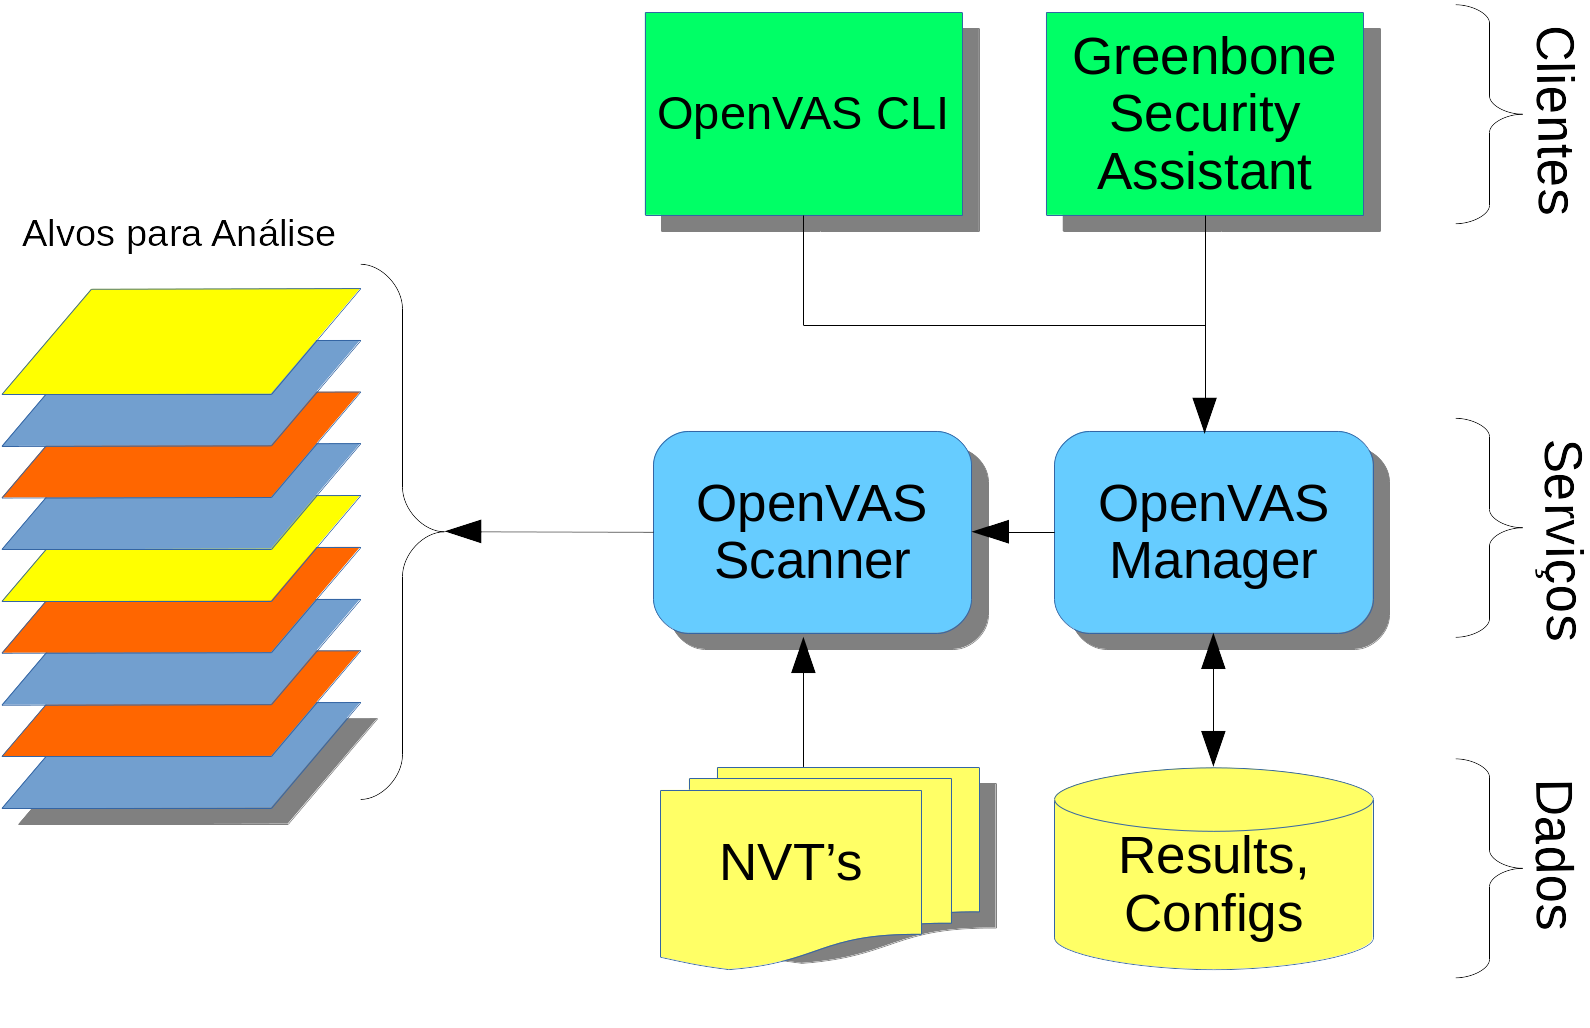
\includegraphics[width=0.90\textwidth]{figuras/Openvas Arquitetura.png}
    \caption{Arquitetura do \gls{OpenVAS} \cite{openvas}.}
    \label{fig:arquitetura:openvas}
\end{figure}

De acordo com \citeonline{vuldec}, a seguir serão descritos os componentes que formam a arquitetura do \gls{OpenVAS}:
\begin{itemize}
    \item \gls{GSA}: Fornece aos usuários uma interface web, na qual os mesmos podem gerenciar as configurações, criar varreduras e visualizar os relatórios de varreduras já executadas.
    \item \gls{OpenVAS} CLI: Cliente \gls{OpenVAS}, responsável por auxiliar o usuário através da interface de linha de comando, permitindo que usuários realizem as mesmas funções providas pelo \gls{GSA}, sem a necessidade de acessar uma interface gráfica.
    \item \gls{OpenVAS} \textit{Manager}: Serviço principal do \gls{OpenVAS}, controla o \textit{scanner} por um protocolo chamado de \gls{OTP}, além de ser responsável por armazenar a configuração e os resultados das varreduras. Também oferece funções adicionais, como por exemplo, agendamento de varreduras, geração de relatórios, entre outras, com uma ferramenta baseada em \gls{XML}, chamada de \gls{OMP}.
    \item \gls{OpenVAS} \textit{Scanner}: Núcleo da arquitetura do \gls{OpenVAS}, executa vários testes chamados de \gls{NVT}, estes testes verificam a presença de vulnerabilidades em sistemas. Os \gls{NVT}s são desenvolvidos utilizando \textit{scripts} da linguagem \gls{NASL}, e assim como o Nessus o \gls{OpenVAS} também possibilita a criação de seus próprios \textit{plugins} (\gls{NVT}) para a verificação de vulnerabilidades.
\end{itemize}

Como já citado anteriormente, o \gls{OpenVAS} é um \textit{framework} composto de vários serviços e ferramentas, segundo \citeonline{allen2014kali}, as ferramentas que compõem o \gls{OpenVAS} são mostradas na tebela~\ref{openvas-table}:
\begin{table}[H]
\centering
\caption{Ferramentas utilizadas pelo \gls{OpenVAS}}
\label{openvas-table}
\begin{tabular}{|l|l|}
\hline
\multicolumn{1}{|l|}{Ferramenta} & \multicolumn{1}{|l|}{Descrição}                                                                                                          \\ \hline
Amap                             & Ferramenta para detecção de protocolo de aplicações                                                                                     \\\hline
Ike-scan                         & \textit{Scanner} para detecção e testes de sistemas IPSec e VPN                                                                          \\\hline
Ldapsearch                       & Extrai informações dos dicionários LDAP                                                                                                 \\\hline
Nikto                            & Realiza análise de vulnerabilidades em servidores web                                                                                   \\\hline
Nmap                             & Realiza uma varredura das portas de um sistema                                                                                          \\\hline
Ovaldi                           & Realiza análise de vulnerabilidades em um sistema                                                                                       \\\hline
pnscan                           & Realiza uma varredura das portas de um sistema                                                                                          \\\hline
Portbunny                        & Realiza uma varredura das portas de um sistema                                                                                          \\\hline
Seccubus                         & Automatiza as varreduras realizadas pelo \gls{OpenVAS}                                                                                \\\hline
SLAD                             & Várias ferramentas de segurança (John-the-Ripper, Chkrootkit, ClamAV,  
\\&Snort,Logwatch, Tripwire, Lsof,Tiger, TrapWatch, e LM-sensors) \\\hline
                          
Snmpwalk                         & Extrai dados dos protocolos SNMP                                                                                                         \\\hline
Strobe                           & Realiza uma varredura das portas de um sistema                                                                                          \\\hline
w3af                             & Realiza ataques em aplicações web
\\ \hline
\end{tabular}
\end{table}

O \gls{OpenVAS} é uma ferramenta completa, podendo ser utilizada para analisar qualquer tipo de rede. Capaz de realizar desde simples varreduras de portas, utilizando ferramentas como Nmap, até quebras de senhas fracas, utilizando john-the-Ripper. Unindo tais características com o fato de ser uma ferramenta de código aberto e possuir uma comunidade forte e crescente, o \gls{OpenVAS} se destaca cada vez mais quando comparados com outros \textit{scanners} do gênero.


\subsection{Nmap}
Network mapper (Nmap), é uma ferramenta grátis e de código aberto, utilizada para monitorar e explorar redes de computadores. O \gls{Nmap} utiliza pacotes \gls{IP} para determinar quais dispositivos estão disponíveis na rede, quais serviços tais dispositivos oferecem, qual são os sistemas operacionais que os dispositivos estão executando, o \gls{MAC} dos dispositivos, entre outras características. O \gls{Nmap} é desenvolvido para monitorar redes com grandes quantidades de dispositivos, porém também funciona  em redes pequenas e/ou dispositivos únicos \cite{lyon2009nmap}.

O \gls{Nmap} também realiza  varreduras das portas de rede dos dispositivos alvos. A partir dessas varreduras são retornados os números das portas de rede, os protocolos de rede utilizados para as comunicações, as aplicações que estão executando e o estado das portas analisadas.

A saída dos dados do \citeonline{nmap} podem ser retornadas de cinco maneiras diferentes,  são elas:
\begin{itemize}
    \item Formato padrão: Todos os dados obtidos da varredura do \gls{Nmap} são mostrados no terminal de execução (\textit{stdout});
    \item Formato normal: Semelhante a saída padrão, porem com menos informações sobre as varreduras realizadas;
    \item Formato \gls{XML}: A varredura é convertida para um arquivo \gls{XML}, é uns dos formatos mais importantes de saída do \gls{Nmap}. O arquivo \gls{XML} pode ser facilmente analisado por programas para extrair informações, pode ser importado para bancos de dados, convertidos em arquivos \gls{HTML}, entres outras opções;
    \item Formato \textit{grep}: As informações sobre um determinado dispositivo são mostradas em apenas uma linha;
    \item Formato \textit{script kiddie}: Alguns caracteres são substituídos por números, não há nada especial neste formado de saída, apenas uma questão visual.
\end{itemize}

Deste modo, o \gls{Nmap} é uma das ferramentas mais poderosas para a análise de redes de computadores, com mais de 100 comandos que podem ser utilizados para realizar varreduras e obter diversas informações a respeito dos dispositivos analisados \cite{lyon2009nmap}.

Para a realização deste trabalho foram escolhida dois \textit{scanners} para serem utilizados, \gls{OpenVAS} e \gls{Nmap}, principalmente pelo fato de não possuírem custos para serem utilizados. Na próxima Seção será explicada a ferramenta de indexação e busca de texto Elasticsearch. 




%---------------------------------------------------%
\section{Elasticsearch}
ElasticSearch é uma ferramenta de busca  de texto de código aberto, desenvolvido na linguagem de programação Java\footnote{\url{https://www.java.com/pt_BR/}} e baseado em Apache Lucene\footnote{\url{https://lucene.apache.org/}}.  ElasticSearch foi desenvolvido com o objetivo de ser distribuído e escalável, tornando-se uma excelente ferramenta para trabalhar com \textit{big data}. É simples de instalar e a configuração padrão é suficiente para ser utilizada sem alterações \cite{Kononenko:2014:MMR:2597073.2597091}.

O Elasticsearch possui algumas características que o diferem do resto dos mecanismos de busca por texto \cite{elastic}, são elas:
\begin{itemize}
    \item Pesquisa e análise de dados em tempo real: Há apenas uma pequena latência do tempo em que um documento é indexado até o tempo em que ele pode ser pesquisado (normalmente um segundo);
    \item Distribuído e escalável: Um servidor Elasticsearch é chamado de nó, dois ou mais nós são chamados de \textit{cluster}. O Elasticsearch pode ser distribuído, analisando grandes quantidades de dados de maneira rápida e prática. A única mudança que precisa ser realizada nos arquivos de configurações é o nome do \textit{cluster}. O Elasticsearch se encarrega de encontrar os nós existentes e distribuir as informações entre os mesmos;
    \item Orientado a documentos: Os dados são armazenados em forma de documentos, um documento tem um tipo e os tipos estão dentro de um Índice. Os documentos são disponibilizados no formato \gls{JSON}, visando maior compatibilidade com várias linguagens de programação;
\end{itemize}


O Elasticsearch é capaz de realizar consultas com tempos muito inferiores quando comparado aos bancos de dados relacionais. Além disso,  possui um sistema de cacheamento, que possibilita que as consultas fiquem ainda mais rápidas a partir do segundo acesso.
O Elasticsearch possui \textit{plugins} que oferecem certas funcionalidades para a ferramenta de busca, visando melhorar a experiência dos usuários, como por exemplo o Kibana, que permite os usuários visualizarem as informações indexadas no motor de busca de forma gráfica e detalhada.
Tais características fazem do Elasticsearch uma poderosa ferramenta de busca, podendo ser utilizado em diversos conjuntos de dados diferentes.

 










%---------------------------------------------------%